\newpage
\section{Билет 3. Вектор перемещения. Связь вектора перемещения и тензоров деформации. Случай малых деформаций. Геометрический смысл компонент. Относительное изменение объема. Уравнение совместности малых деформаций.}

\begin{center}
	\textit{\underline{Вектор перемещения. Связь вектора перемещения и тензоров деформации.}}
\end{center}

\begin{figure}[H]
	\centering
	\noindent\centering{
		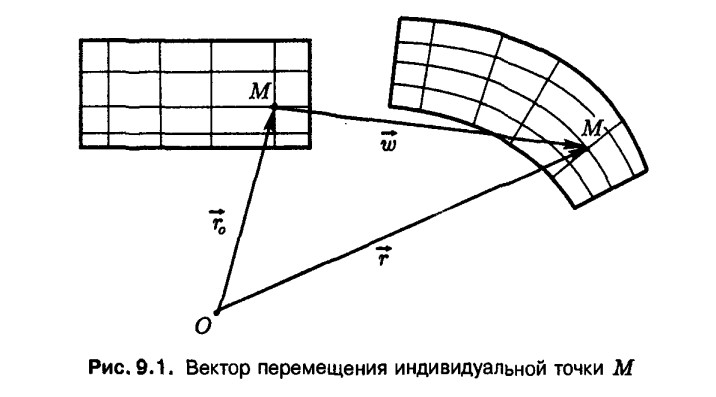
\includegraphics[width=10cm]{3/3_1.jpg}
	}
	\label{fig1}
\end{figure}

Вектор перемещений $\vec w = \vec r - \vec r_0$ - вектор, соединяющий точки, где находится индивидуальная точка среды $М$ в начальном и конечном состояниях среды.	
Лагранжевы координаты точки - её неизменные параметры, так что и в начальном, и в конечном состояниях это $\xi^i$. Продифференцируем по ним вектор перемещений:
$$
\dd{\vec w}{\xi^i} = \dd{\vec r}{\xi^i} - \dd{\vec r_0}{\xi^i} = \hat{\vec{e_i}} - \arcsup{\vec{e_i}}, \quad \text{т.е.}\quad 
\hat{\vec{e_i}} = \arcsup{\vec{e_i}} +\dd{\vec w}{\xi^i}\quad \left(\text{или} \quad  \arcsup{\vec{e_i}} = \hat{\vec{e_i}} - \dd{\vec w}{\xi^i}\right)
$$
Тогда
$$
\varepsilon_{ij} = \frac{1}{2}(\hat{g_{ij}} - \arcsup{g_{ij}}) = \frac{1}{2}((\hat{\vec{e_i}}, \hat{\vec{e_j}}) - (\arcsup{\vec{e_i}}, \arcsup{\vec{e_j}})) = \frac{1}{2}\left(\left(\arcsup{\vec{e_i}} + \dd{\vec w}{\xi^i} , \arcsup{\vec{e_j}} + \dd{\vec w}{\xi^j} \right) - (\arcsup{\vec{e_i}}, \arcsup{\vec{e_j}})\right) = \frac{1}{2}\left( \arcsup{\vec{e_i}}\dd{\vec w}{\xi^j} + \arcsup{\vec{e_j}}\dd{\vec w}{\xi^i} + \dd{\vec w}{\xi^i} \dd{\vec w}{\xi^j}\right)
$$

Вектор $w$ разложим по, соответственно, ковариантному и контравариантному базису: 
$\vec w = \arcsup{w}^k\arcsup{\vec e}_k$  и $\vec w = \arcsup{ w}_k\arcsup{\vec e}^k$. Тогда $\dd{\vec w}{\xi^i} = \nabla_i\arcsup{w}^k\arcsup{\vec e}_k = \nabla_i\arcsup{w}_k\arcsup{\vec e}^k$.

Учитывая, что $(\vec e^k,\vec e_i) = \delta_i^k$, подставим разложение $w$:
$$
\varepsilon_{ij} = \dfrac{1}{2}(\nabla_j\arcsup{w}_k(\arcsup{\vec e}^k, \arcsup{\vec e}_i) + \nabla_i\arcsup{w}_k(\arcsup{\vec e}^k, \arcsup{\vec e}_j) + \nabla_i\arcsup{w}^k \nabla_j\arcsup{w}_l(\arcsup{\vec e}_k, \arcsup{\vec e}^l)) = \dfrac{1}{2}(\nabla_j\arcsup{w}_i + \nabla_i\arcsup{w}_j + 
\nabla_i\arcsup{w}^k \nabla_j\arcsup{w}_k)
$$
(Здесь следует подставлять координаты начальной точки $\vec w = w^i(x_0^k)e_i(x_0^k)$, а можно вывести аналогичное $\varepsilon_{ij} = \dfrac{1}{2}(\nabla_j\hat {w}_i + \nabla_i\hat {w}_j + 
\nabla_i\hat {w}^k \nabla_j\hat {w}_k)$ и подставлять координаты конечной точки $\vec w = w^i(x^k)e_i(x^k)$).

\begin{center}
	\textit{\underline{Случай малых деформаций.}}
\end{center}

В случае $\nabla_i {w}^k \ll 1$, или $\nabla_i {w}_k\nabla_j {w}^k \ll \nabla_i {w}_k$, получим тензор малых деформаций $\varepsilon_{ij} = \dfrac{1}{2}(\nabla_j {w}_i + \nabla_i {w}_j)$.

$\hat{\vec{e_i}} = \arcsup{\vec{e_i}} +\dd{\vec w}{\xi^i} = \hat{\vec{e_i}} = \arcsup{\vec{e_i}} +\nabla_i\arcsup{w}^k\arcsup{\vec e}_k = (\delta_i^k + \nabla_i\arcsup{w}^k)\arcsup{\vec{e_i}}$, откуда видно, что из малости производных перемещений следует малость деформаций. Обратное неверно, так как относительные перемещения могут быть большими даже при малых деформациях, если относительные повороты отрезков не малы (тело, размеры которого во всех направлениях не одного порядка: пластинки, оболочки, стержни). Согнем металлическую линейку, она практически не растягивается, но ее элементы поворачиваются друг относительно друга:
\begin{figure}[H]
	\centering\noindent{
		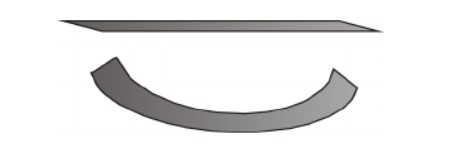
\includegraphics[width=10cm]{3/3_2.jpg}
	}
	\label{fig2}
\end{figure}

\begin{center}
	\textit{\underline{Геометрический смысл компонент.}}
\end{center}

По определению скалярного произведения: $\hat g_{ij} = (\hat{\vec{e_i}}, \hat{\vec{e_j}}) = |\hat{\vec{e_i}}||\hat{\vec{e_j}}|\cos\psi_{ij}, \quad \arcsup g_{ij} = (\arcsup{\vec{e_i}}, \arcsup{\vec{e_j}}) = |\arcsup{\vec{e_i}}||\arcsup{\vec{e_j}}|\cos\arcsup\psi_{ij}$, где $\psi_{ij}, \arcsup\psi_{ij}$ - углы между векторами базиса лагранжевой системы координат в начальном и конечном состояниях. Отсюда
$$
\varepsilon_{ij} = \frac{1}{2}(|\hat{\vec{e_i}}||\hat{\vec{e_j}}|\cos\psi_{ij} - |\arcsup{\vec{e_i}}||\arcsup{\vec{e_j}}|\cos\arcsup\psi_{ij}).
$$

Коэффициент относительного удлинения малого отрезка: $e = \dfrac{ds - ds_0}{ds_0}$

\noindent
\parbox[b][4cm][t]{10mm}{
	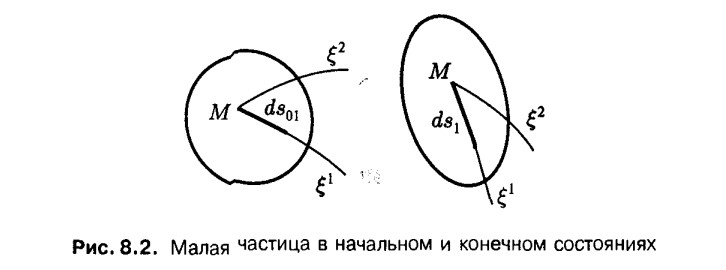
\includegraphics[height=3.75cm]{3/3_3.jpg}}
\hfill
\parbox[b][4cm][t]{68mm}{
	Бесконечно малый вектор вдоль $\xi^1: d\vec r_0 = d\xi^1\arcsup{\vec{e_1}}$. 
	
	Его длина $ds_{01} = d\xi^1|\arcsup{\vec{e_1}}|$.
	
	При деформации перейдет в вектор: $d\vec r = d\xi^1\hat{\vec{e_1}}$. 
	
	Его длина $ds_{1} = d\xi^1|\hat{\vec{e_1}}|$.
	
	
}

\hfill

$e_1 = \dfrac{ds_1 - ds_{01}}{ds_{01}} = \dfrac{d\xi^1|\hat{\vec{e_1}}| - d\xi^1|\arcsup{\vec{e_1}}|}{d\xi^1|\arcsup{\vec{e_1}}|} = \dfrac{|\hat{\vec{e_1}}|}{|\arcsup{\vec{e_1}}|} - 1$. Аналогично, $e_i = \dfrac{|\hat{\vec{e_i}}|}{|\arcsup{\vec{e_i}}|} - 1$, $i = 1,2,3$.

Отсюда $|\hat{\vec{e_i}}| = (1+e_i)|\arcsup{\vec{e_i}}|$. Тогда

$$
\varepsilon_{ij} = \dfrac{1}{2}((1+e_i)(1+e_j)\cos\psi_{ij} - \cos\arcsup\psi_{ij})|\arcsup{\vec{e_i}}||\arcsup{\vec{e_j}}|.
$$

\begin{itemize}	
	\item При $i = j$: Т.к. $\psi_{ij} = 0 = \arcsup\psi_{ij}$, то 
	$\varepsilon_{ii} = \dfrac{1}{2}((1+e_i)^2 - 1)|\arcsup{\vec{e_i}}|^2 = (e_i + \dfrac{1}{2}e_i^2)|\arcsup{\vec{e_i}}|^2$.
	Если отсчетная система декартова (т.е. $|\arcsup{\vec{e_i}}| = 1$): $\varepsilon_{ii} = (e_i + \dfrac{1}{2}e_i^2)$. Если, к тому же, деформации малы (т.е. $\dfrac{1}{2}e_i^2 \ll e_i$), то $\varepsilon_{ii} = e_i$. (т.е.в случае малых деформаций диагональные элементы - это коэффициенты относительного удлинения материальных отрезков, лежащих вдоль координатных осей).
	\item При $i \not= j$: Если отсчетная система декартова (т.е. $|\arcsup{\vec{e_i}}| = 1, \arcsup\psi_{ij} = \dfrac{\pi}{2}$), введем $\chi_{ij} = \arcsup\psi_{ij} - \psi_{ij} = \dfrac{\pi}{2} - \psi_{ij}$. Тогда $\varepsilon_{ij} = \dfrac{1}{2}(1+e_i)(1+e_j)\sin{\chi_{ij}}$. Если, к тому же, деформации малы (т.е. $e_i \ll 1, \sin \chi_{ij} \approx \chi_{ij}$): $\varepsilon_{ij} = \dfrac{1}{2}\chi_{ij}$. (т.е. в случае малых деформаций внедиагональные элементы - это половина изменения угла между материальными отрезками, лежащими вдоль координатных осей).
\end{itemize}

Если $\varepsilon_{ij} = 0$, то $\chi_{ij} = 0$ и $\psi_{ij} = \dfrac{\pi}{2}$, т.е. в результате деформации углы между координатными осями остаются ортогональныим.

\begin{center}
	\textit{\underline{Относительное изменение объема.}}
\end{center}

Возьмем в качестве начальной лагранжевой системы главную систему для тензора Грина, т.е. 
$$
\arcsup g_{ij} = 
\begin{pmatrix} 
1 & 0 & 0 \\
0 & 1 & 0 \\
0 & 0 & 1 
\end{pmatrix},
\varepsilon_{ij} = 
\begin{pmatrix} 
\varepsilon_{11} & 0 & 0 \\
0 & \varepsilon_{22} & 0 \\
0 & 0 & \varepsilon_{33}
\end{pmatrix} = 
\begin{pmatrix} 
\arcsup\varepsilon_{1} & 0 & 0 \\
0 & \arcsup\varepsilon_{2} & 0 \\
0 & 0 & \arcsup\varepsilon_{3}
\end{pmatrix}
\Rightarrow
\hat g_{ij} = 
\begin{pmatrix} 
1+2\arcsup\varepsilon_{1} & 0 & 0 \\
0 & 1+2\arcsup\varepsilon_{2} & 0 \\
0 & 0 & 1+2\arcsup\varepsilon_{3}
\end{pmatrix}
$$
(последняя матрица получена из $\varepsilon_{ij} = \frac{1}{2}(\hat{g_{ij}} - \arcsup{g_{ij}})$). Т.е. в деформированном состоянии лагранжева система ортогональна, $\varepsilon_{ij}$ - диагональна.

Отсюда 
$$ |\hat{\vec{e_i}}| = \sqrt{g_{ii}} = \sqrt{1 + 2\arcsup\varepsilon_{i}} = (1+e_i)|\arcsup{\vec{e_i}}| = (1+e_i)
$$
Рассмотрим малую частицу среды, имевшую в начальном состоянии форму прямоугольного параллелепипеда, построенного на векторах $d\xi^1\arcsup{\vec{e_1}}$, $d\xi^2\arcsup{\vec{e_2}}$, $d\xi^3\arcsup{\vec{e_3}}$. Его объем $dV_0 = d\xi^1d\xi^2d\xi^3$. Т.к. $\varepsilon_{ij} = 0$ при $i \not= j$, то деформированный параллелепипед тоже прямоугольный с ребрами $d\xi^1\hat{\vec{e_1}}$, $d\xi^2\hat{\vec{e_2}}$, $d\xi^3\hat{\vec{e_3}}$. Его объем $dV = |\hat{\vec{e_1}}||\hat{\vec{e_2}}||\hat{\vec{e_3}}|d\xi^1d\xi^2d\xi^3$.
\begin{figure}[H]
	\centering\noindent{
		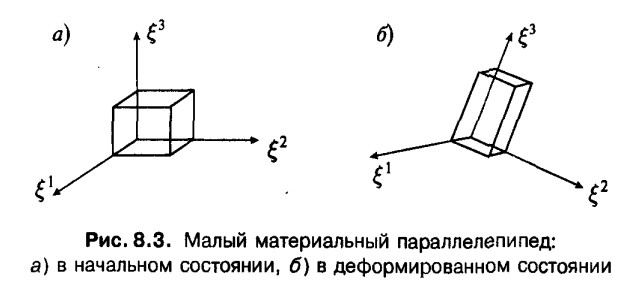
\includegraphics[width=10cm]{3/3_4.jpg}
	}
	\label{fig4}
\end{figure}
Относительное изменение объема $\theta = \dfrac{dV - dV_{0}}{dV_{0}} = \sqrt{(1+2\arcsup\varepsilon_{1})(1+2\arcsup\varepsilon_{2})(1+2\arcsup\varepsilon_{3})} - 1 = (1+e_1)(1+e_2)(1+e_3) - 1$. В случае малых деформаций: $\theta \approx e_1 + e_2 + e_3 = \sum\varepsilon_{ii} = \sum\nabla_iw^i = div {\vec w}$.


\begin{center}
	\textit{\underline{Уравнение совместности малых деформаций.}}
\end{center}

В декартовой системе $\varepsilon_{ij} = \dfrac{1}{2}\left(\dd{w_i}{x^j}+ \dd{w_j}{x^i}\right)$. Используя обозначения $\dd{\varepsilon_{ij}}{x^k} = \varepsilon_{ij, k}$, продифференцируем:
\begin{gather*}
\varepsilon_{ij, kl} = \dfrac{1}{2}(w_{i,jkl} + w_{j,ikl}) \\
\varepsilon_{kl, ij} = \dfrac{1}{2}(w_{k,lij} + w_{l,kij}) \\
\varepsilon_{il, jk} = \dfrac{1}{2}(w_{i,ljk} + w_{l,ijk}) \\
\varepsilon_{jk, il} = \dfrac{1}{2}(w_{j,kil} + w_{k,jil}) \\
\end{gather*}
Из непрерывности перемещений: $\varepsilon_{ij, kl} + \varepsilon_{kl, ij} - \varepsilon_{il, jk} - \varepsilon_{jk, il} = 0$. Здесь 81 уравнение (рассматривается трехмерное пространство), из которых только 6 независимые (в силу симметричности компонент тензора деформации и равенства смешанных производных):
\begin{gather*}
2\varepsilon_{12, 12} = \varepsilon_{11, 22} + \varepsilon_{22, 11} \\
2\varepsilon_{13, 13} = \varepsilon_{11, 33} + \varepsilon_{33, 11} \\
2\varepsilon_{23, 23} = \varepsilon_{22, 33} + \varepsilon_{33, 22} \\
\varepsilon_{11, 23} = \dd{}{x^1}(-\varepsilon_{23, 1} + \varepsilon_{13, 2} + \varepsilon_{12, 3}) \\
\varepsilon_{22, 13} = \dd{}{x^2}(-\varepsilon_{13, 2} + \varepsilon_{21, 3} + \varepsilon_{23, 1}) \\
\varepsilon_{33, 12} = \dd{}{x^3}(-\varepsilon_{12, 3} + \varepsilon_{23, 1} + \varepsilon_{13, 2})
\end{gather*}